%=========================================
% Archivo:
% capitulos/11_resultados.tex
%=========================================

\chapter{Resultados y Análisis}

Este capítulo presenta los resultados experimentales obtenidos durante la evaluación comparativa de las cinco implementaciones desarrolladas: Secuencial, Multicore, OpenMP, MPI y CUDA. El análisis se centra en el tiempo de ejecución, speedup, eficiencia y escalabilidad de cada paradigma de paralelización.

Todos los experimentos fueron ejecutados sobre el mismo conjunto de datos y bajo las mismas condiciones, garantizando la comparabilidad objetiva de los resultados.

%--------------------------------------------------------

\section{Comparación de Tiempos de Ejecución}

La Figura \ref{fig:time_comparison} presenta la comparación de los tiempos de ejecución obtenidos por cada implementación.

\begin{figure}[H]
\centering
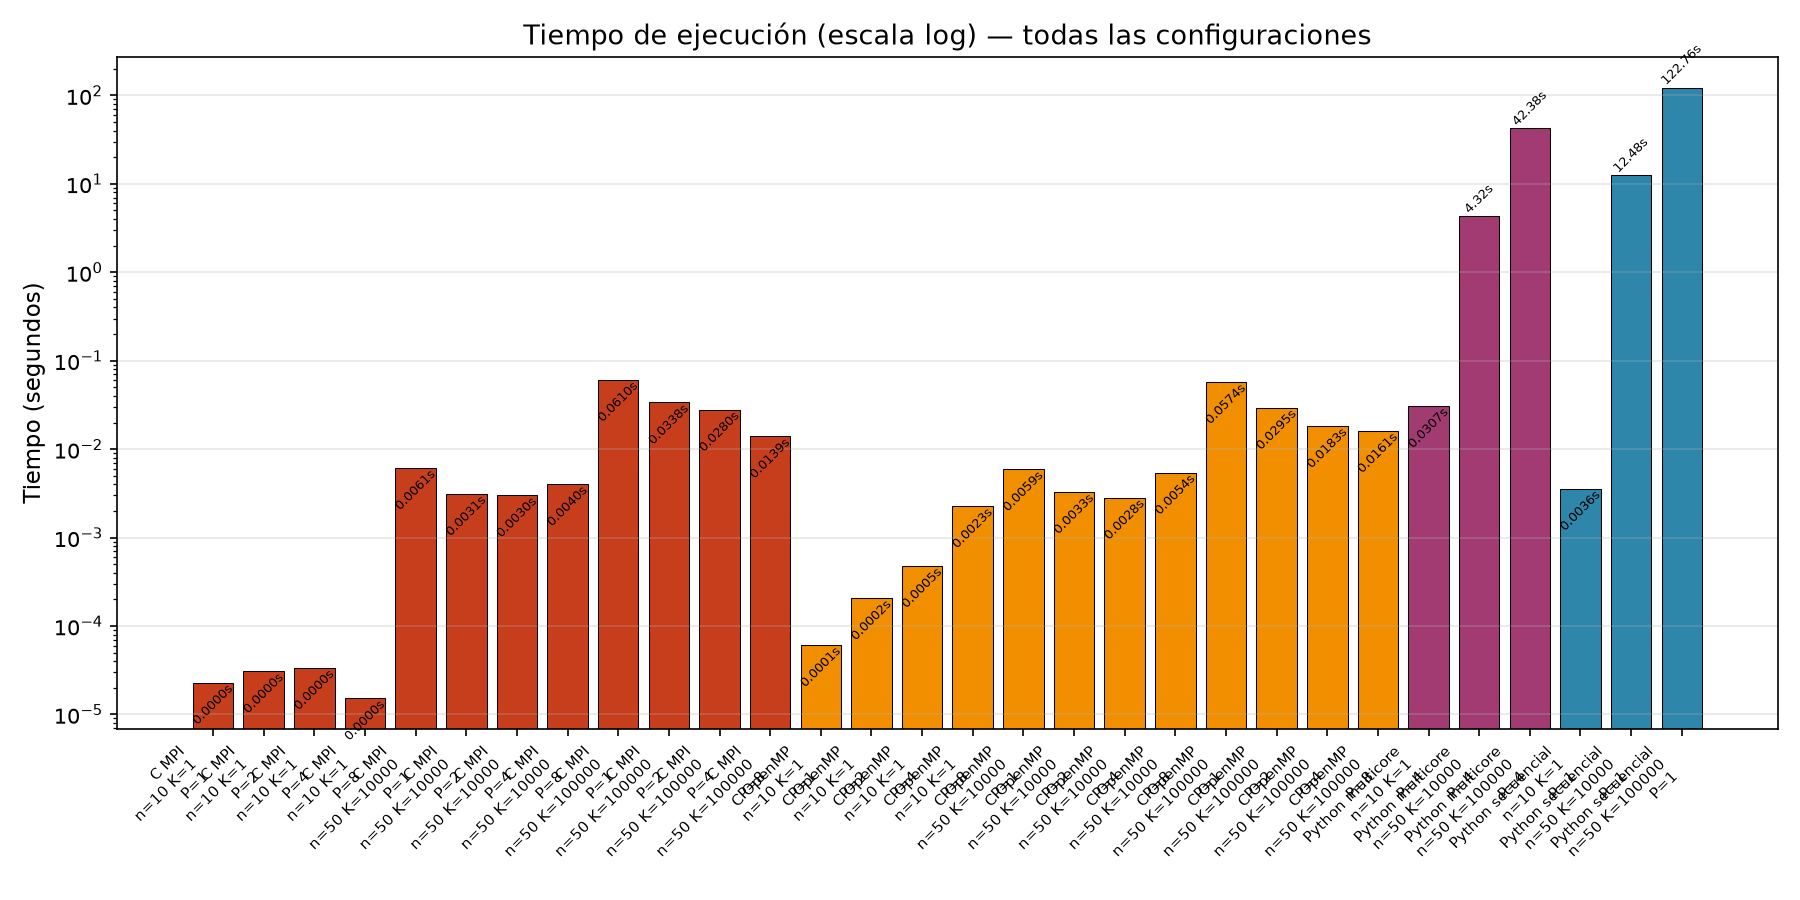
\includegraphics[width=.95\textwidth, height=0.45\textheight, keepaspectratio]
{figuras/graficas/time_comparison.png}
\caption{Comparación de tiempos de ejecución entre implementaciones.}
\label{fig:time_comparison}
\end{figure}

%--------------------------------------------------------

\section{Speedup respecto a la Implementación Secuencial en Python}

La Figura \ref{fig:speedup_vs_python} muestra el speedup obtenido por cada implementación paralela respecto a la versión secuencial en Python.

\begin{figure}[H]
\centering
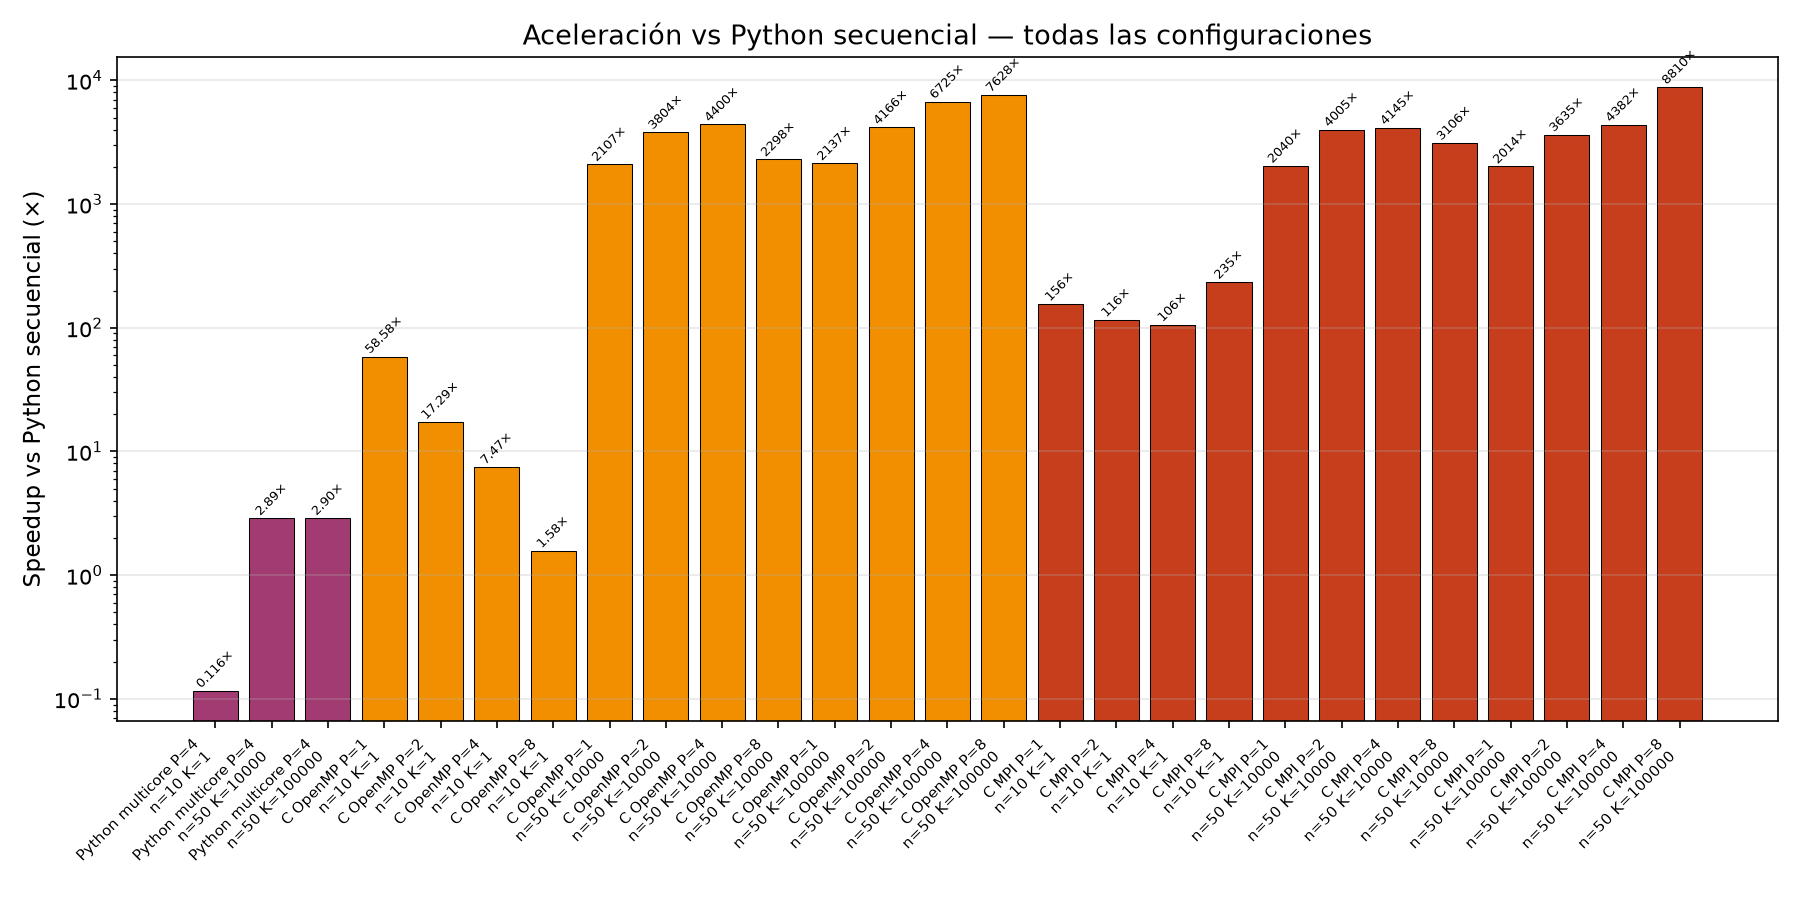
\includegraphics[width=.95\textwidth, height=0.45\textheight, keepaspectratio]
{figuras/graficas/speedup_vs_python.png}
\caption{Speedup de cada implementación respecto a la versión secuencial en Python.}
\label{fig:speedup_vs_python}
\end{figure}

%--------------------------------------------------------

\section{Escalabilidad y Speedup}

La Figura \ref{fig:speedup_scalability} presenta el comportamiento del speedup en función del número de unidades de procesamiento utilizadas.

\begin{figure}[H]
\centering
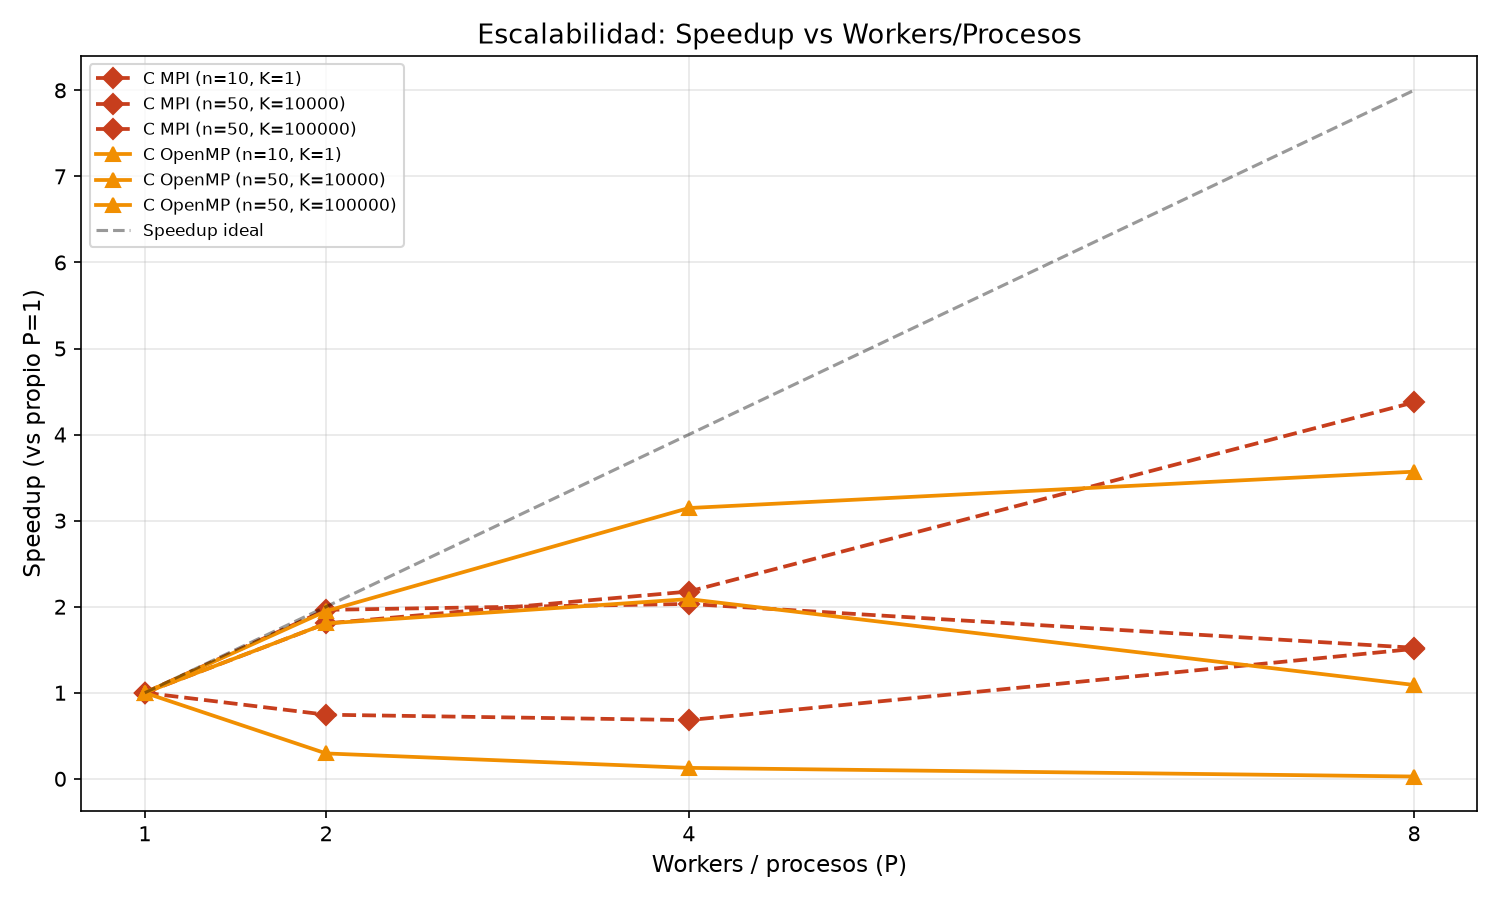
\includegraphics[width=.95\textwidth, height=0.45\textheight, keepaspectratio]
{figuras/graficas/speedup_scalability.png}
\caption{Speedup y escalabilidad en función del número de unidades de procesamiento.}
\label{fig:speedup_scalability}
\end{figure}

%--------------------------------------------------------

\section{Eficiencia}

La Figura \ref{fig:efficiency} presenta la eficiencia de cada implementación paralela, definida como el cociente entre el speedup obtenido y el número de unidades de procesamiento utilizadas.

\[
E = \frac{S}{P} = \frac{T_s}{P \times T_p}
\]

\begin{figure}[H]
\centering
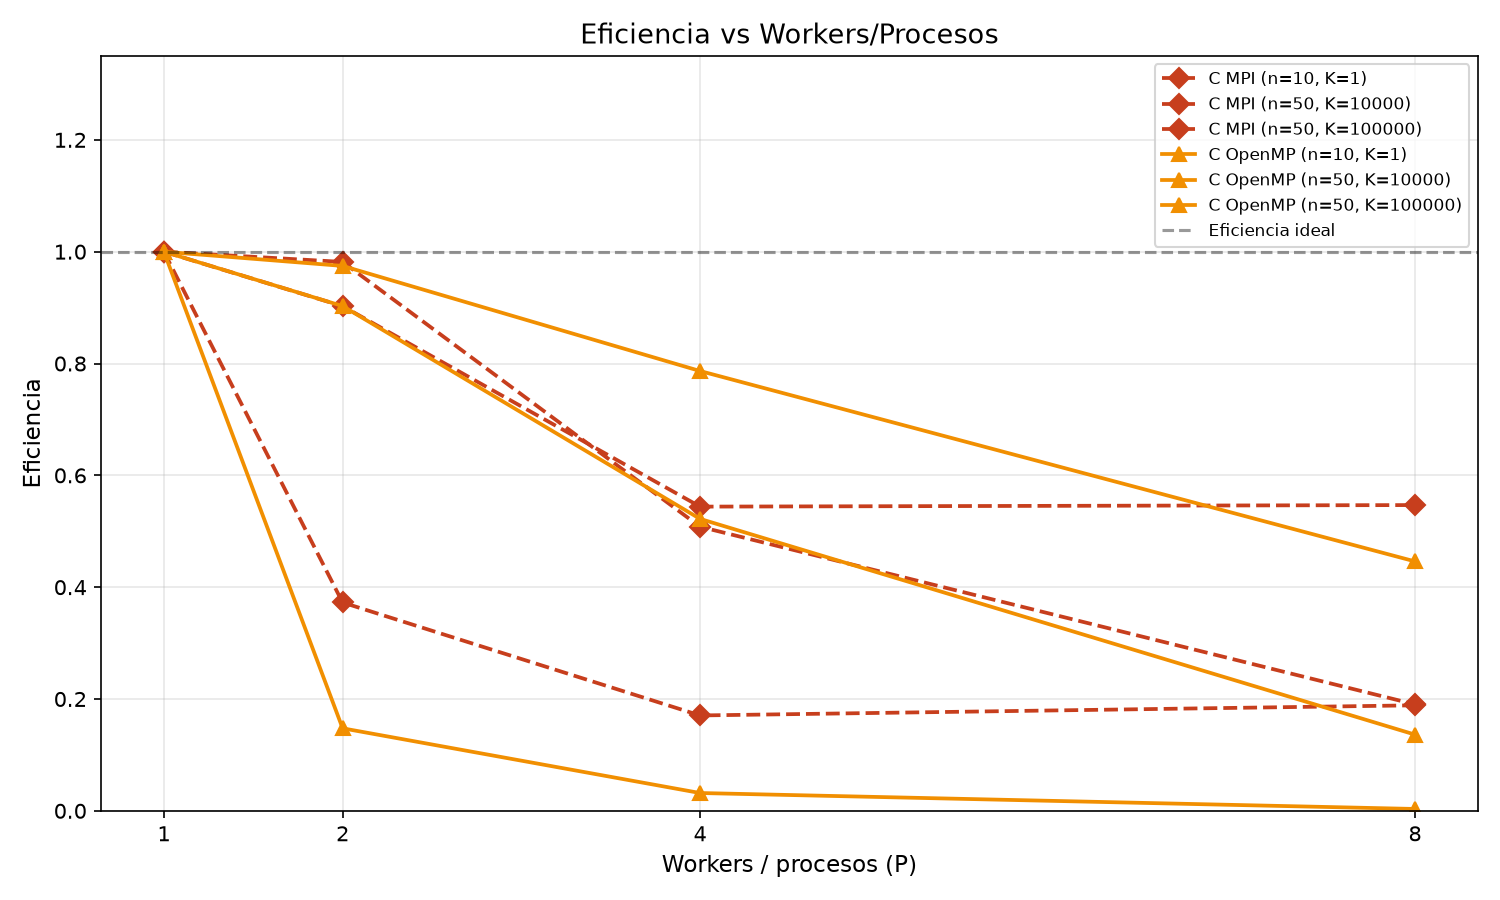
\includegraphics[width=.95\textwidth, height=0.45\textheight, keepaspectratio]
{figuras/graficas/efficiency.png}
\caption{Eficiencia de cada implementación en función del número de unidades de procesamiento.}
\label{fig:efficiency}
\end{figure}

%--------------------------------------------------------

\section{Throughput}

La Figura \ref{fig:throughput} presenta el throughput de cada implementación, expresado como el número de candidatos evaluados por segundo.

\begin{figure}[H]
\centering
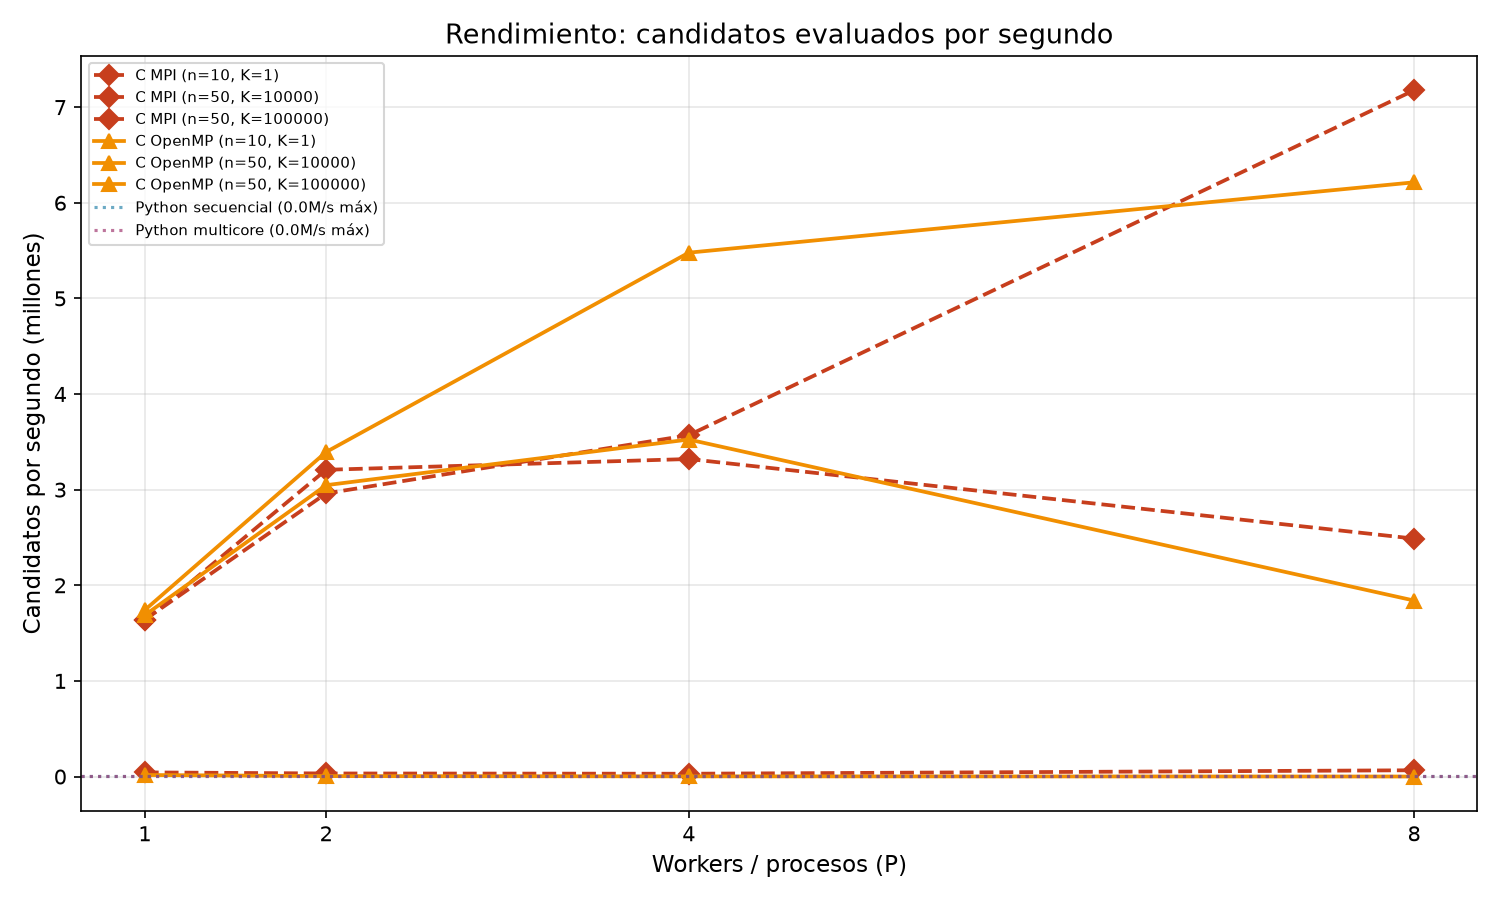
\includegraphics[width=.95\textwidth, height=0.45\textheight, keepaspectratio]
{figuras/graficas/throughput.png}
\caption{Throughput de cada implementación expresado en candidatos por segundo.}
\label{fig:throughput}
\end{figure}

%--------------------------------------------------------

\section{Resumen Comparativo}

La Figura \ref{fig:summary_table} resume los principales indicadores de rendimiento obtenidos por cada implementación durante los experimentos.

\begin{figure}[H]
\centering
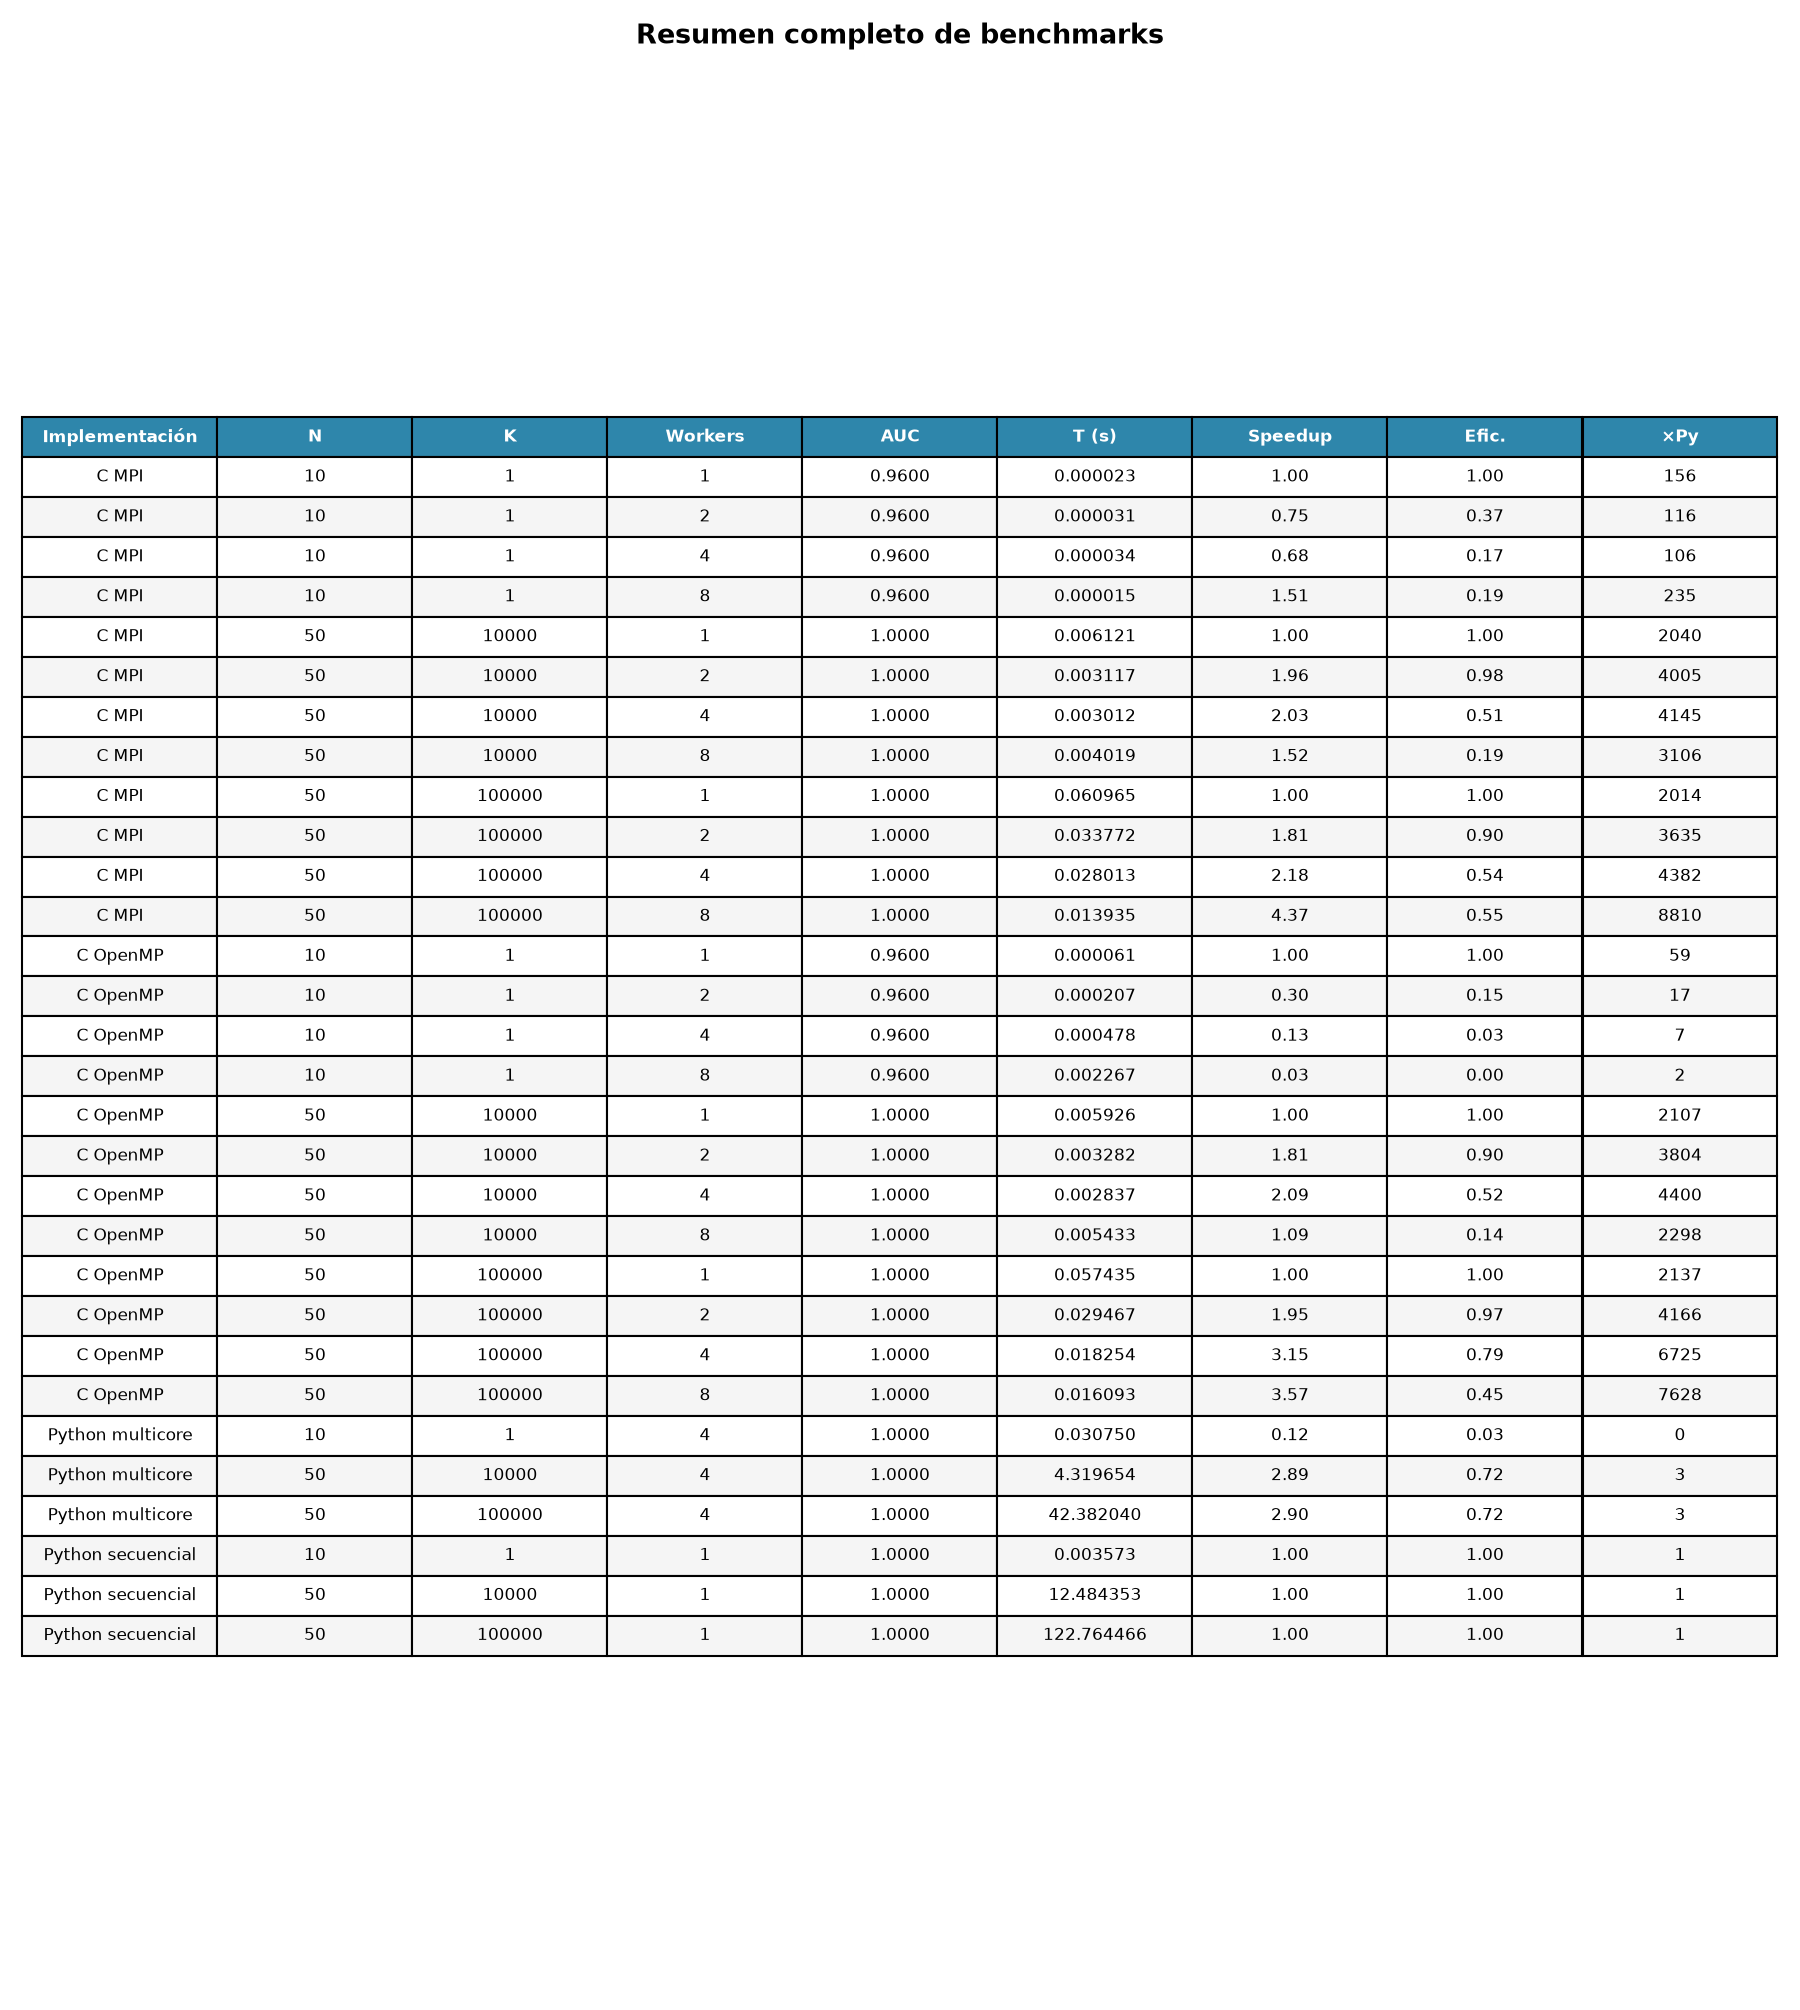
\includegraphics[width=.95\textwidth, height=0.45\textheight, keepaspectratio]
{figuras/graficas/summary_table.png}
\caption{Resumen comparativo de los indicadores de rendimiento por implementación.}
\label{fig:summary_table}
\end{figure}

%--------------------------------------------------------

\section{Análisis General}

Los resultados obtenidos permiten observar que todas las implementaciones paralelas superan a la versión secuencial en tiempo de ejecución, manteniendo el mismo valor óptimo de ROC-AUC.

El speedup crece conforme aumenta el número de unidades de procesamiento, siendo CUDA la implementación con mayor aceleración para volúmenes grandes de candidatos debido al paralelismo masivo disponible en la GPU.

OpenMP y MPI presentan un comportamiento similar en entornos de un solo nodo, con OpenMP mostrando menor overhead para problemas de tamaño moderado.

La eficiencia disminuye a medida que se incrementa el número de unidades de procesamiento, comportamiento esperado y consistente con la Ley de Amdahl, dado que una fracción del algoritmo permanece inherentemente secuencial.